\documentclass[a4paper,11pt]{article}
\usepackage[utf8]{inputenc}
\usepackage{fullpage}
\usepackage{amsmath,amssymb,amsfonts}
\usepackage{tikz}
%\usepackage{hyperref}
%\usepackage{color}

\title{}
\author{}
\date{}

\newcommand{\tr}{\operatorname{tr}}
\newcommand{\diag}{\operatorname{diag}}
\newcommand{\Res}{\mathop{Res}}
%\numberwithin{equation}{section}

\begin{document}
%\maketitle

\begin{enumerate}
\item\label{item:1} Solve wave equation \(u_{tt}-u_{xx}=0\) on \(\mathbb{R}\) with the following initial conditions \[u_t(0,x)=|1-x^2|\theta_H(1-x^2), \qquad u(0,x)=0,\] where \(\theta_H(x)=0\) for  \(x\le 0\), \(\theta_H(x)=1\) for \(x>0\).

Plot this solution for some values of \(t\).

\item\label{item:2} Solve wave equation \(u_{tt}-u_{xx}=0\) on \(\mathbb{R}_{>0}\) with the following initial and boundary conditions
\[u_t(0,x)=0,\qquad u(0,x)=\sin^2(2\pi x)\theta_H(1-|x-2|), \quad u(t,0)= \frac12\sin^2(2\pi t)\theta_H(1-|t-2|)\]

Plot this solution for some values of \(t\).

\item\label{item:3} Find the Fourier transform of the function \(\frac{1}{e^{2\pi i x}-1/2}\) on a circle \(x\sim x+1\).

\item\label{item:4} Find the Fourier transform of the function \(\frac{1}{\cos(2\pi x)-\cosh(2\pi a)}\) on a circle \(x\sim x+1\).

\item\label{item:5} Find the Fourier transform of the function \(\frac{1}{x^2+1}\) on \(\mathbb{R}\).

\item\label{item:6} Find the Fourier transform of the function \(\frac{\sin x}{x^2+1}\) on \(\mathbb{R}\).

\item\label{item:7} Find the Fourier transform of the function \(\frac{\sin x}{x}\) on \(\mathbb{R}\).

\item\label{item:8} Solve the equation
\[u_{tt}-2u_{xx}-u_{tx}=0, \qquad u_t(0,x)=0, \qquad u(0,x)=(1-x^2)\theta_H(1-x^2).\]

\item\label{item:9} Find the Fourier transform of \(\frac1{\cosh x}\).

\begin{itemize}
\item One option is to consider the difference of the two integral, over \(\mathbb{R}\) and over \(\mathbb{R}+2\pi i\): first to compare it with the original integral, and second compute by residues.
\item Another option is to close the contour and compute it as a sum of residues.
\end{itemize}

\item\label{item:10} Solve the equation
\[u_{tt}-u_{xx} = f(t,x), \qquad u_t(0,x)=0, \qquad u(0,x)=0, \qquad f(t,x) = |1-|x||\theta_H(1-|x|)\theta_H(t(1-t)).\]
Plot this solution, e.g., for \(t=10\).

\item\label{item:11} Solve the equation
\[u_t-u_{xx}=0, \qquad u(0,x)=e^{-(x-a)^2}\]

\item\label{item:12} Solve the equation
\[u_t-u_{xx}=0, \qquad u(0,x)=\sin x\]

\item\label{item:13} Solve the equation
\[u_t-u_{xx}=0,\quad x\ge 0,\qquad |u(-\infty,x)|<\infty , \qquad |u(t,+\infty)|<\infty,\quad u(t,0)=\sin t\]

\item\label{item:14} Solve the equation
\[u_{tt}-u_{xx}-u_{yy}=\delta(x)\delta(y)\theta_H(t(1-t)), \quad t>0, \qquad u(0,x,y)=u_t(0,x,y)=0.\quad\]

\item\label{item:15} Find a formula for \(\mathrm{P}\frac1{f(x)}\), analogous to \(\delta(f(x))=\sum\limits_{f(x_n)=0}\frac1{|f'(x_n)|}\delta(x-x_n)\).

\item\label{item:16} Solve the equation
\[u_t(t,\vec{r})-\Delta u(t,\vec{r})=0, \quad \vec{r}\in \mathbb{R}^d,\qquad u(0,\vec{r})=\vec{r}e^{-(\vec{r}-\vec{r}_0)^2}.\]

\item\label{item:18} Solve the equation
\[\Delta u(x,y)=0, \quad x^2+y^2\le 1, \quad u(\cos\phi,\sin\phi) = \sin 2\phi.\]

\item\label{item:19} Solve the equation
\[\partial_tu(t,x)-u_{xx}(t,x)=\sin x\sin t, \quad u(0,x)=0\]
in the limit \(t\to \infty\).

\item\label{item:20} Solve the equation
\[
\Delta u(x,y,z)=0,\quad x^2+y^2+z^2\le 1, \quad u(\sin\theta\cos\phi,\sin\theta\cos\phi,\cos\theta)=\cos 2\theta.
\]

\item\label{item:21} Solve the equation
\[
\Delta u(x,y)=\delta(x-x_0)\delta(y-y_0), \quad \arg(x+iy)\in (0,\pi/3), \quad u(r\cos \frac{\pi}{3}, r\sin \frac{\pi}{3})=u(r,0)=0.
\]

\item\label{item:22} Expand each component of the vector
\[
(\sin\theta\cos\phi,\sin\theta\sin\phi,\cos\theta)P_1(\cos\theta)
\]
in the basis of spherical functions.

\item\label{item:23} Find solutions of the Sturm-Liouville problem
\[
u''(x)=-\lambda u(x), \quad u(0)=0, \quad u'(1)=0.
\]
Check that corresponding \(u_n(x)\) form a complete system (expand an arbitrary function in this basis and check that the inverse transformation reproduces it).

\item\label{item:44} Find radially symmetric solution of the Helmholtz equation
\[\Delta u(r)+u(r)=0,\]
regular at \(r=0\), in two- and three-dimensional space.

\end{enumerate}

\newpage

\section*{Answers}

\begin{enumerate}
\item\label{item:17} \(u(t,x)=\frac12(\phi(x+t)-\phi(x-t))\), where \(\phi(x)=\int_0^x (1-y^2)dy = x-x^3/3, |x|<1\), and \(\phi(x)=2/3 \operatorname{sign}x, |x|>1\).

The plot for \(t=5\):
\begin{center}
\begin{tikzpicture}[scale=1,
declare function = {phi(\x)=(\x<-1)*(-2/3)+and(\x>=-1, \x<=1)*(\x-\x*\x*\x/3)+(\x>1)*(2/3);}]
\draw[->](-7,0)--(7,0) node[below]{\(x\)};
\draw[->](0,-1)--(0,3) node[right]{\(u(5,x)\)};
\draw[domain=-7:7,samples=100,thick,blue] plot (\x,{phi(\x+5)-phi(\x-5)});
\node at (0.4,1.6){\(2/3\)};
\draw(-4,4/3+0.1)--(-4,-0.1) node[below]{\(-4\)};
\draw(4,4/3+0.1)--(4,-0.1) node[below]{\(4\)};
\draw(-6,+0.1)--(-6,-0.1) node[below]{\(-6\)};
\draw(6,+0.1)--(6,-0.1) node[below]{\(6\)};
\node at (0.2,-0.25){\(0\)};
\end{tikzpicture}
\end{center}

\item\label{item:24} \(u(t,x)=\frac12\sin^2(2\pi (x-t))\theta_H(1-|x-t-2|)+\frac12\sin^2(2\pi (x+t))\theta_H(1-|x+t-2|)\)

\item\label{item:26} \(\frac1{e^{2\pi ix}-1/2}=\sum_{n=0}^{\infty}2^{-n}e^{-2\pi i n x}\).

\item\label{item:27} \(\frac{1}{\cos 2\pi x - \cosh 2\pi a}=-\sum_{n\in \mathbb{Z}} \frac{e^{2\pi i n x - 2\pi a |n|}}{\sinh 2 \pi a}\)

\item\label{item:28} \(\frac1{x^2+1}=\int_{-\infty}^{\infty}\frac12 e^{-|p|+i p x}dp\)

\item\label{item:29} \(\frac{\sin x}{x^2+1}=\int_{-\infty}^{\infty} \frac{i}{4}\left(e^{-|p+1|}-e^{-|p-1|} \right)e^{i p x} dp\)

\item\label{item:30} \(\frac{\sin x}{x}=\int \frac12 \left( \theta_H(p+1)-\theta_H(p-1) \right) e^{i p x}dx\)

\item\label{item:31} \(u(t,x)=\frac1{3}\phi(x+2t)+\frac{2}{3}\phi(x-t),\quad \phi(x)=(1-x^2)\theta_H(1-x^2)\)

\item\label{item:32} \(\frac1{\cosh x}=\int_{-\infty}^{\infty} \frac{e^{i p x}}{2\cosh \frac{\pi p}{2}} dp\)

\item\label{item:33} \(u(t,x)=\frac12 \int_0^{\min(t,1)}dt'\int_{x-t+t'}^{x+t-t'}dx'(1-|x'|)\theta_H(1-|x'|)\),

\(t>1\): \(u(t,x)=\frac12 \int_0^1 dt' \left(\phi(x+t-t')-\phi(x-t+t')\right)=\)

\(=\frac12 \left(-\Phi(x+t-1)+\Phi(x+t)-\Phi(x-t+1)+\Phi(x-t) \right)\),

where \(\phi(x)=\int_0^xdy (1-|y|)\theta_H(1-|y|) = \operatorname{sign}(y) \max\left(|y|-\frac12 y^2,\frac12\right)\)

and \(\Phi(x)=\int_0^xdy \phi(y) = \max(\frac12 x^2-\frac1{6}|x|^3,\frac12 |x| - \frac1{6})\)

The plot for \(t=10\):
\begin{center}
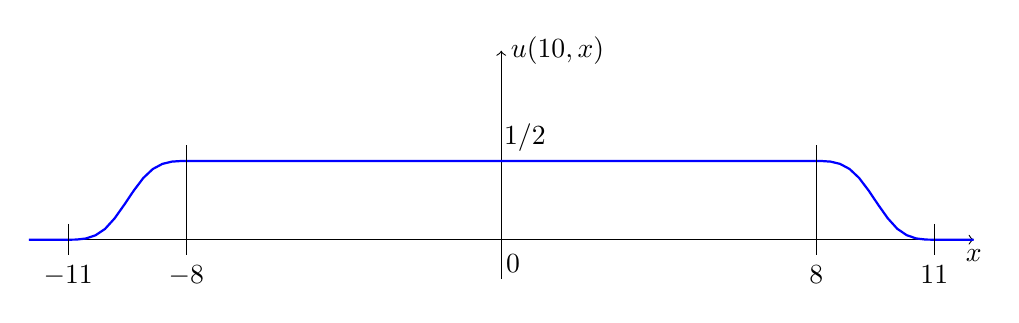
\begin{tikzpicture}[xscale=0.5,yscale=2,
declare function = {phi(\x)=1/2*max(1/2*\x*\x-1/6*\x*\x*abs(\x),1/2*abs(\x)-1/6);}]
\draw[->](-12,0)--(12,0) node[below]{\(x\)};
\draw[->](0,-1/4)--(0,1.2) node[right]{\(u(10,x)\)};
\draw[domain=-12:12,samples=100,thick,blue] plot (\x,{-phi(\x+9)+phi(\x+10)-phi(\x-9)+phi(\x-10)});
\node at (0.6,1/2+0.15){\(1/2\)};
\draw(-8,1/2+0.1)--(-8,-0.1) node[below]{\(-8\)};
\draw(8,1/2+0.1)--(8,-0.1) node[below]{\(8\)};
\draw(-11,+0.1)--(-11,-0.1) node[below]{\(-11\)};
\draw(11,+0.1)--(11,-0.1) node[below]{\(11\)};
\node at (0.3,-0.15){\(0\)};
\end{tikzpicture}
\end{center}

\item \label{item:34}\(u(t,x)=\frac{e^{-\frac{(x-a)^2}{1+4t}}}{\sqrt{1+4t}}\)

\item\label{item:35} \(u(t,x)=e^{-t} \sin x\)

\item\label{item:35} \(u(t,x)=e^{-x/\sqrt{2}}\sin \left(t-x/\sqrt{2}\right)\)

\item\label{item:25} \(u(t,x,y)=\phi(t,\sqrt{x^2+y^2})-\phi(t-1,\sqrt{x^2+y^2})\),
where \(\phi(t,r)=\theta_H(t-r)\log \frac{\sqrt{t^2-r^2}+t}{r}\)

\item\label{item:36} \(\mathrm{P} \frac1{f(x)} = \left(\frac1{f(x)}-\sum_i \frac1{f'(x_i)(x-x_i)} \right) + \sum_i \frac1{f'(x_i)} \mathrm{P} \frac1{x-x_i}\)

\item\label{item:37} \(u(t,\vec{r}) = \frac{e^{-(\vec{r}-\vec{r}_0)^2} \left(\vec{r}+4 t \vec{r}_0\right)}{(1+4t)^{3/2}}\)

\item\label{item:38} \(u(x,y) = 2 x y\)

\item\label{item:39} \(u(t,x) = \frac12 \sin x \left(\sin t-\cos t \right)\)

\item\label{item:40} \( u(x,y,z) = \frac1{3}\left( 4z^2-2x^2-2y^2-1 \right)\)

\item\label{item:41} \(u(z,\bar{z})=\frac1{4\pi}\log\left|\frac{(z^3-z_0^3)}{(z^3-\bar{z}^3)}\right|\), where \(z=x+iy\).

\item\label{item:42} \(\frac1{3}\left(Y_{2,1}(\theta,\phi)+Y_{2,-1}(\theta,\phi),i(Y_{2,1}(\theta,\phi)-Y_{2,-1}(\theta,\phi)),2Y_{2,0}(\theta,\phi)+1\right)\),
where we fixed for simplicity \(Y_{2,\pm 1}(\theta,\phi)=P_2^1(\cos\theta)e^{\pm i\phi}\), \(Y_{2,0}=P_2(\cos\theta)\)

\item\label{item:43} \(f_n(x)=\sqrt{2}\sin\pi(n+1/2)x\), \((f_n,f_m)=\delta_{n,m}\), \(\tilde{u}_n=\int_0^1 f_n(x) u(x)\), \(u(x)=\sum_{n=1}^{\infty} \tilde{u}_n f_n(x)\),
\(\sum_{n=0}^{\infty}e^{-\epsilon n}f_n(x)f_n(y)=\delta_{\epsilon}(x,y)\). \(\delta_0(x,y)=0\) for \(x\neq y\). \(\delta_{\epsilon}(x,x+\delta)\sim \frac{\epsilon}{\pi^2\delta^2+\epsilon^2}\), so \(\delta_{\epsilon}(x,y)\to \delta(x-y)\).

\item\label{item:45} d=2: \(u(r)=J_0(r)\), d=3: \(u(r)=\frac{\sin r}{r}\).

\end{enumerate}

\end{document}
